\begin{center}
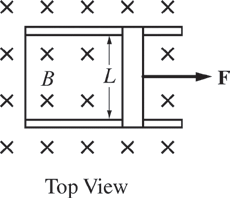
\includegraphics[scale=0.5]{images/img-009-029.png}
\end{center}

% Multiple Choice Question 32
\begin{questions}\setcounter{question}{31}\question
A metal rod of length $L$ that can slide on horizontal frictionless metal rails is moved through a uniform magnetic field of magnitude $B$ that is perpendicular to the rails, as shown in the figure above. The other ends of the rails are connected by a wire to form a circuit of resistance $R$. An external force of magnitude $F$ is applied to the rod so that the rod maintains a constant speed $v$. What is the power supplied by the force?

\begin{oneparchoices}
\choice $\dfrac{B^{2} L^{2} v}{R}$
\choice $\dfrac{B^{2} L^{2} v}{R^{2}}$
\choice $\dfrac{B^{2} L v^{2}}{R}$
\choice $\dfrac{B^{2} L^{2} v^{2}}{R}$
\choice $\dfrac{B^{2} L v^{3}}{R}$
\end{oneparchoices}\end{questions}

